\documentclass[11pt,a4paper]{article}
\usepackage[margin=25mm,headheight=15pt]{geometry}
\usepackage[T1]{fontenc}
\usepackage[utf8]{inputenc}
\usepackage{lmodern,microtype,amsmath,amssymb,amsthm,mathtools}
\usepackage{graphicx,booktabs,array,tabularx,longtable,enumitem,xcolor,fancyhdr,xurl,hyperref}
\definecolor{teal}{HTML}{185B58}
\definecolor{muted}{HTML}{516466}
\hypersetup{colorlinks=true,linkcolor=teal,urlcolor=teal,pdftitle={Euler Congruences: Visual Guide, Final Strengthened Edition},pdfauthor={Komorebi P.},bookmarksnumbered=true}
\setlength{\parindent}{0pt}
\setlength{\parskip}{.5em}
\setlength{\emergencystretch}{2em}
\setlist{itemsep=2pt,topsep=4pt}
\allowdisplaybreaks[1]
\pagestyle{fancy}\fancyhf{}
\fancyhead[L]{\small\scshape\color{muted}Euler congruences / Chapter IX}
\fancyhead[R]{\small\scshape\color{muted}Visual guide}
\fancyfoot[L]{\small Komorebi P.}\fancyfoot[R]{\thepage}
\renewcommand{\headrulewidth}{.4pt}

% Operation Komorebi: shared publication profile.
\usepackage{komorebi-publication}
\renewcommand{\KomorebiTitle}{Euler Congruences}
\renewcommand{\KomorebiSubtitle}{Completion, factorial strengthening, and sharp dyadic geometry}
\renewcommand{\KomorebiSeries}{Chapter IX}
\renewcommand{\KomorebiKind}{Visual studies}
\renewcommand{\KomorebiEdition}{}
\renewcommand{\KomorebiShortTitle}{Chapter IX}
\renewcommand{\KomorebiTitleSize}{38}
\renewcommand{\KomorebiTitleLeading}{43}
\renewcommand{\KomorebiProfile}{atlas}
\renewcommand{\KomorebiOrientation}{portrait}
\KomorebiSetup
\begin{document}
\KomorebiCover
\KomorebiOpeningNote{{\color{teal}\hrule height .7pt}\medskip
This guide explains the indexing, valuation gains, exact periods, and remaining boundaries through exact arithmetic and theorem-derived figures. The main text supplies the proofs. The formal companion supplies the formal source and evidence map.}

\hypersetup{pageanchor=false}

\hypersetup{pageanchor=true}
\pagenumbering{roman}
{\small\setlength{\parskip}{0pt}\tableofcontents}
\clearpage
\pagenumbering{arabic}
\section{The object: rows, degrees, and normalization}

The visual guide accompanies \emph{Euler Congruences: Completion, Factorial Strengthening,
and Sharp Dyadic Geometry}. It makes the indexing,
precision gains, and boundaries of the results visible. The main text contains
the proofs. The separate Lean guide records which statements are already
formalized and which belong to the new mathematical extension.

\begin{figure}[ht]
\centering
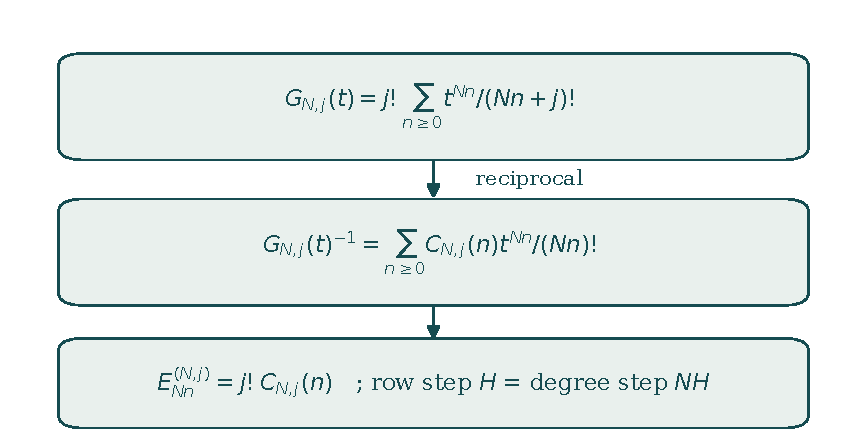
\includegraphics[width=.96\linewidth]{../figures/normalization.pdf}
\caption{The actual reciprocal series is the source of every coefficient in
this guide. The factorial normalization changes valuations as well as the
constant term.}
\end{figure}

There are two coefficient conventions, and they must stay distinct:
\[
 C_{N,j}(0)=1,
 \qquad E_0^{(N,j)}=j!,
 \qquad
 v_2(E_{Nn}^{(N,j)})=v_2(C_{N,j}(n))+v_2(j!).
\]
The last equality uses $v_2(0)=+\infty$. Congruences of dyadic rational numbers
mean membership in the corresponding ideal of $\mathbb Z_2$. A displayed
rational denominator is invertible modulo $2^r$ when it is odd.

\begin{center}
\begin{tabular}{lll}
\toprule
Symbol & Meaning & At rank four \\
\midrule
$n$ & packed row index & Euler degree $4n$ \\
$H$ & positive row step & Euler degree step $4H$ \\
$k$ & number of differences & order $k$, independent of $n$ \\
$j$ & address within a section & $0,1,2,3$ \\
\bottomrule
\end{tabular}
\end{center}

For example, $C_{4,1}(1)=-1/5$ and $C_{4,1}(2)=121/45$.
Their difference is $26/9$, of valuation one. The row difference joins Euler
degrees $4$ and $8$.

\clearpage
\section{What the original conjecture asked}

Nishibuchi's Conjecture 3.9 concerns a prime $p$, a positive integer $m$ with
$m\mid p-1$ or $m=2$, and every address $0\le j<mp$. Put
\[
 N=mp, \qquad q=\operatorname{lcm}(2,p-1).
\]
It asserts $p$-adic integrality of the actual generalized Euler coefficients and
eventual periodicity at every precision:
\[
 \text{for every }r\ge1,\quad
 E_{mpn+qp^r}^{(mp,j)}\equiv E_{mpn}^{(mp,j)}\pmod {p^r}
 \quad\text{for all sufficiently large }n.
\]
The completed theorem gives the explicit sufficient threshold $n\ge r$ in
every permitted branch. Its formal capstone is the theorem named
\texttt{NishibuchiCompletion.conjecture\_3\_9}. No conjectural flatness premise
is supplied to that theorem.

\begin{center}
\begin{tabular}{llll}
\toprule
Prime branch & Allowed $m$ & $q$ & Row step for the original shift \\
\midrule
$p=2$ & $1$ & $2$ & $2^r$ \\
$p=2$ & $2$ & $2$ & $2^{r-1}$ \\
$p$ odd & $m\mid p-1$ & $p-1$ & $\dfrac{p-1}{m}p^{r-1}$ \\
\bottomrule
\end{tabular}
\end{center}

For odd primes, $m=2$ is already in the divisor branch. The conversion is exact:
\[
 N\left(\frac qm p^{r-1}\right)=qp^r.
\]
At $p=2,m=2$, the original conjectured Euler-degree shift $2^{r+1}$ is the row
step $2^{r-1}$ for the rank-four sequence.

The source already contains special cases. In particular, Nishibuchi's
Proposition 3.10 treats the rank-four address-zero dyadic period from row zero
and an eventual cubic case. The completion covers the full quantified
conjecture. The new dyadic work then removes starting-row restrictions from
higher differences and determines substantially more precise laws.

The conjecture's primary source is Yuta Nishibuchi, \emph{$p$-adic Congruences of
Generalized Euler Numbers and Relations to Even Zeta Values},
arXiv:2605.10677v2, revised 1 June 2026. The statement above uses that version's
normalization and actual Euler degrees.

\clearpage
\section{Removing the starting-row threshold}

At rank four the earlier completed estimate was
$v_2(\Delta_H^k C_j(n))\ge\min(k,n)$. The strengthened theorem reaches every
starting row, including $n=0$, and every order, including $k>n$.

\begin{figure}[ht]
\centering
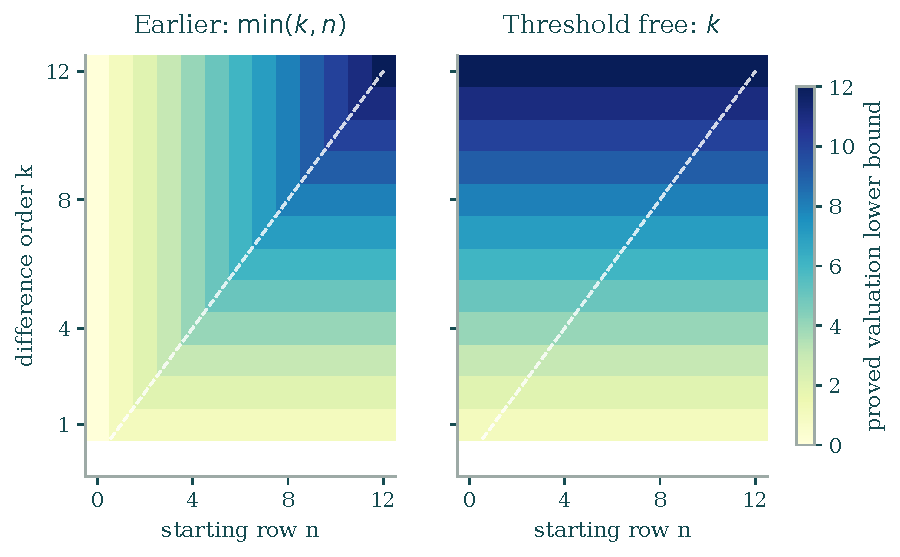
\includegraphics[width=\linewidth]{../figures/threshold.pdf}
\caption{Unit-step lower bounds on a finite display window. Each colored cell
is obtained from a proved formula, rather than from sampled coefficients.
The dashed line indicates $k=n$.}
\end{figure}

For \emph{every} dyadic section size $N=2^a$, $a\ge0$, every permitted address,
and all positive steps,
\[
 v_2\!\left(\Delta_{H_1}\cdots\Delta_{H_k}C_{N,j}(n)\right)
 \ge k+\sum_{\nu=1}^k v_2(H_\nu),
 \qquad n\ge0.
\]
The corresponding statement for $E_{Nn}^{(N,j)}$ adds $v_2(j!)$.

The proof acts on the full factorial-scaled power series before it extracts a
packed row. This avoids the old extraction constraint $k\le n$. Reciprocal
induction controls the unique term with the highest inverse order in the
commuting product expansion. All other terms are covered by the preceding
induction stages.

The figure displays the gain at unit step. An even step contributes additional
precision, and the theorem permits different steps in the same difference.

\clearpage
\section{Each step contributes its own precision}

Write $Sf(n)=f(n+1)$ and $\Delta_H=S^H-1$. Mixed differences commute. Their
exact finite expression is
\[
 \Delta_{H_1}\cdots\Delta_{H_k}f(n)
 =\sum_{A\subseteq\{1,\ldots,k\}}
 (-1)^{k-|A|}
 f\!\left(n+\sum_{i\in A}H_i\right).
\]
Repeated subset offsets are combined with their signed multiplicities.

\begin{figure}[ht]
\centering
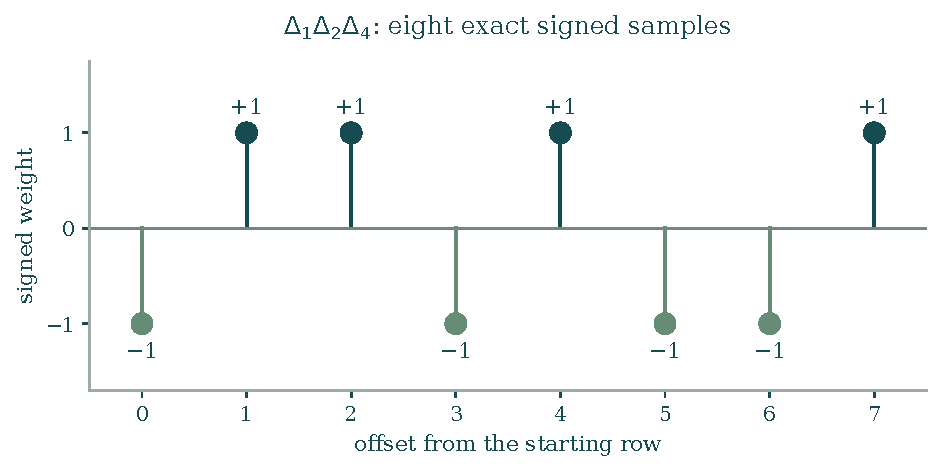
\includegraphics[width=\linewidth]{../figures/mixed_stencil.pdf}
\caption{For steps $(1,2,4)$ all eight offsets are distinct. This is an exact
signed stencil, rather than an approximate derivative.}
\end{figure}

For this stencil, the general dyadic bound is
\[
 3+v_2(1)+v_2(2)+v_2(4)=6.
\]
At rank four the factorial theorem improves it to seven for addresses zero
and one. Exact rational evaluation gives
$v_2(\Delta_1\Delta_2\Delta_4 C_0(0))=7$.
The order is odd, so the mixed-step equality criterion also proves this
valuation at \emph{every} starting row.

There is a prime-power extension. For $N=p^a$, $a\ge1$, the sign-corrected
operator is
\[
 T_H=S^H-(-1)^H,
 \qquad
 v_p\!\left(T_{H_1}\cdots T_{H_k}E^{(N,j)}(n)\right)
 \ge v_p(j!)+\sum_{i=1}^k\bigl(1+v_p(H_i)\bigr).
\]
Here $E^{(N,j)}(n)=E_{Nn}^{(N,j)}$. For an odd prime, an ordinary first
difference need not have positive valuation: at address zero its first two
normalized values are $1$ and $-1$, with difference $-2$. The sign correction
is therefore essential to this prime-power theorem.

\clearpage
\section{The final rank-four congruence}

For $n\ge0$, $k\ge1$, and $H\ge1$, the actual Euler coefficients satisfy
\[
 \sum_{i=0}^k(-1)^{k-i}\binom ki
 E_{4(n+iH)}^{(4,j)}
 \equiv0\pmod {2^{\,v_2(k!)+k v_2(H)+A_j(k)}},
\]
where
\[
\begin{aligned}
 A_0(k)=A_1(k)&=k,\\
 A_2(k)&=\max\{k+4,\ 2k+\lfloor k/2\rfloor+1\},\\
 A_3(k)&=k+2.
\end{aligned}
\]

\begin{figure}[ht]
\centering
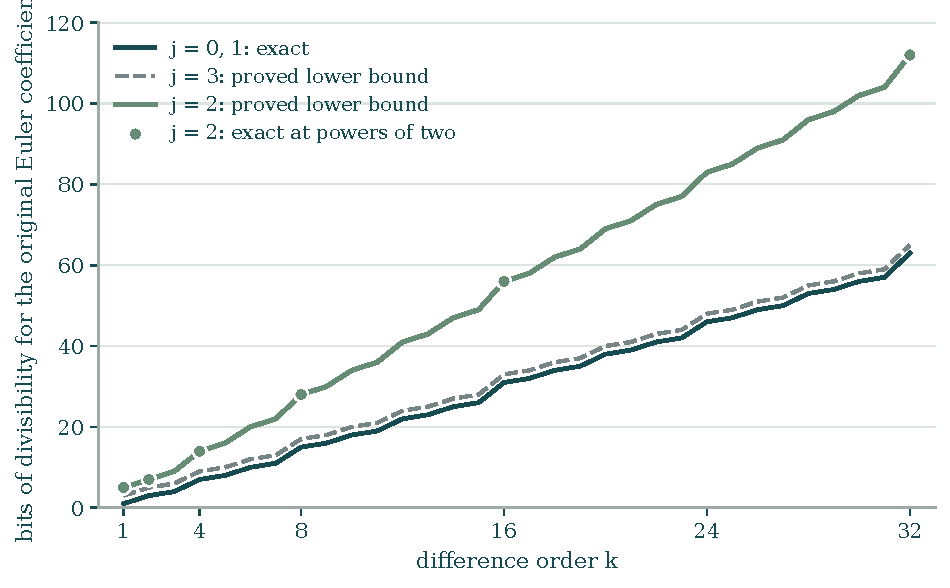
\includegraphics[width=\linewidth]{../figures/final_exponents.pdf}
\caption{The exponent of the final Euler congruence at unit step. The address
zero and one curve is exact at every order. Marked address-two orders are
universally exact. The other displayed address-two and address-three values
are proved lower bounds.}
\end{figure}

At a common step with $v_2(H)=s$, add $ks$ to every displayed exponent. Thus a
doubling of the step gains one additional bit \emph{per difference}, rather
than one bit for the whole expression.

This statement combines two different proved bounds at address two. A lower
bound is not automatically an exact valuation: divisibility may be stronger
at unmarked orders or at particular starting rows.

\clearpage
\section{Why address two has a different slope}

The normalized address-two sequence obeys both
\[
\begin{aligned}
 v_2(\Delta_{H_1}\cdots\Delta_{H_k}C_2(n))
 &\ge k+v_2(k!)+3+\sum_i v_2(H_i),\\
 v_2(\Delta_{H_1}\cdots\Delta_{H_k}C_2(n))
 &\ge2k+v_2(k!)+\lfloor k/2\rfloor+\sum_i v_2(H_i).
\end{aligned}
\]
Their maximum supplies the useful envelope.

\begin{figure}[ht]
\centering
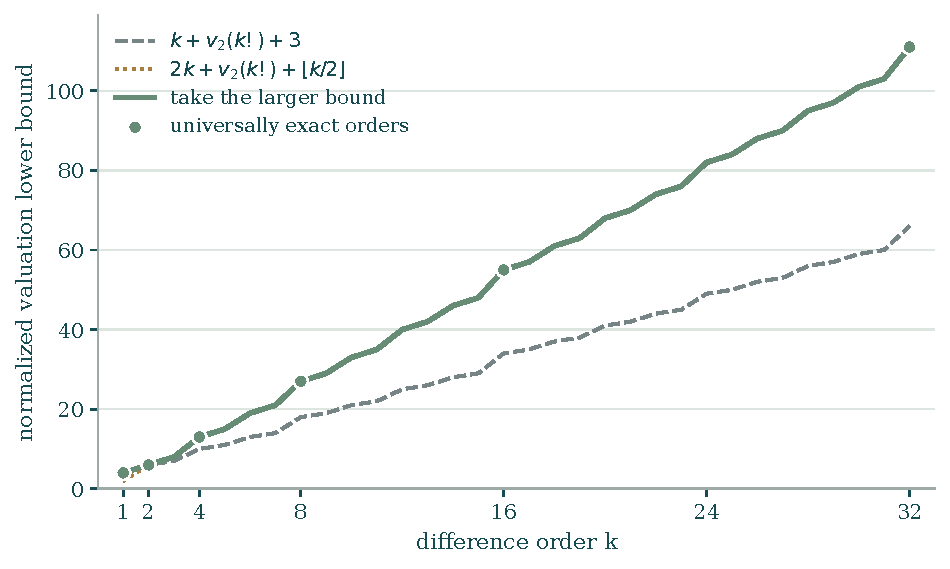
\includegraphics[width=\linewidth]{../figures/address_two_envelope.pdf}
\caption{Normalized address-two precision. The paired filtration controls the
large-order slope. At order one the constant-surplus bound is stronger.}
\end{figure}

For every base row and every positive step list, equality is proved when
$k$ is a power of two:
\[
 v_2(\Delta_{H_1}\cdots\Delta_{H_k}C_2(n))
 =V_2(k)+\sum_i v_2(H_i),
\]
with $V_2(1)=4$, $V_2(2)=6$, and
$V_2(k)=2k+v_2(k!)+k/2$ for $k=2^r\ge4$.
The infinite marked family establishes sharpness at unbounded orders.

For original Euler coefficients add one, since $v_2(2!)=1$.
The extra $\lfloor k/2\rfloor$ comes from a paired divided-power filtration in
the Bernoulli transformation. It does not arise by fitting the plotted points.

\clearpage
\section{When mixed steps attain the baseline}

For addresses $j=0,1$, put
\[
 V=k+v_2(k!)+\sum_i v_2(H_i),
 \qquad q=\#\{i:H_i\text{ is even}\}.
\]
The valuation equals $V$ exactly when $k$ is odd or $q$ is even.

\begin{center}
\begin{tabular}{lll}
\toprule
Order parity & Number of even steps & Conclusion \\
\midrule
$k$ odd & either parity & exact valuation $V$ \\
$k$ even & $q$ even & exact valuation $V$ \\
$k$ even & $q$ odd & valuation at least $V+1$ \\
\bottomrule
\end{tabular}
\end{center}

\begin{figure}[ht]
\centering
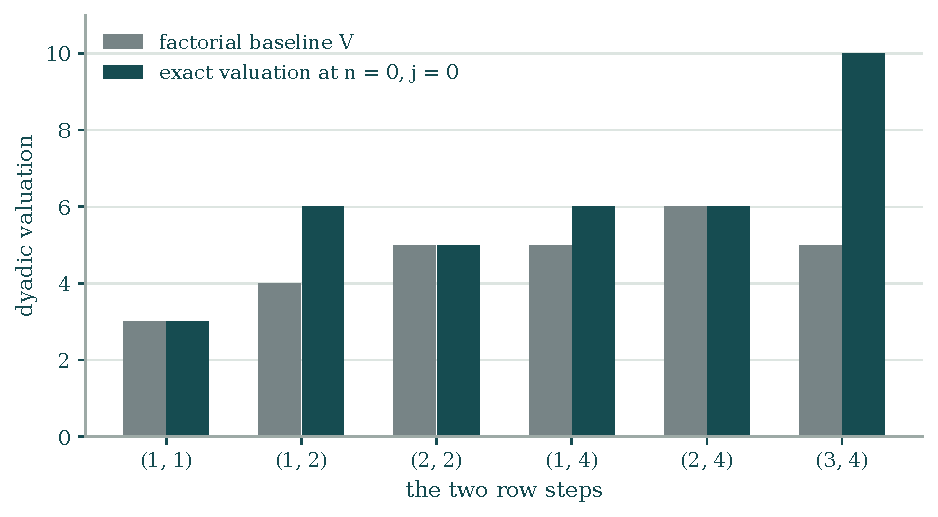
\includegraphics[width=\linewidth]{../figures/mixed_cancellation.pdf}
\caption{Exact rational examples at order two and base zero. Strict cases
show why the factorial baseline cannot always be called an equality for
mixed steps. The universal parity criterion is proved separately.}
\end{figure}

For instance,
\[
 \Delta_1\Delta_2 C_0(0)=-33728,
 \qquad v_2(-33728)=6,
 \qquad V=4.
\]
Cancellation removes the leading term, and here it removes two bits beyond
the baseline. The parity theorem proves strictness in this case. It does not
give a complete formula for the further depth.

With a common step, $q$ is either zero or $k$. Consequently the exceptional
parity never occurs, and the homogeneous address-zero/one formula is always
exact.

\clearpage
\section{First differences determine an exact metric}

All four rank-four sequences satisfy the sharp first-difference law
\[
 v_2(C_j(n+H)-C_j(n))=v_2(H)+b_j,
 \qquad b=(1,1,4,2).
\]
For the actual Euler coefficients this becomes
\[
 v_2(E_{4(n+H)}^{(4,j)}-E_{4n}^{(4,j)})=v_2(H)+B_j,
 \qquad B=(1,1,5,3).
\]
Both laws hold at every starting row and every positive integer step.

\begin{figure}[ht]
\centering
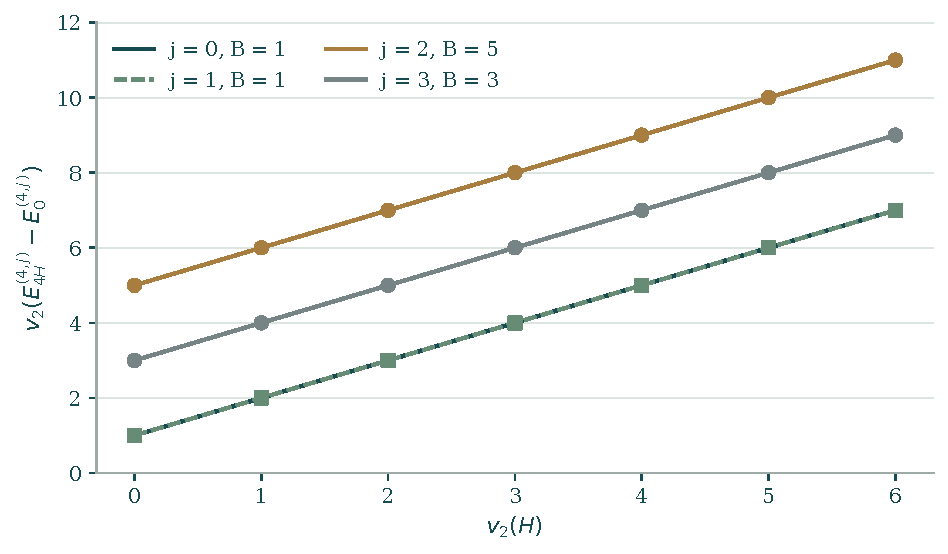
\includegraphics[width=\linewidth]{../figures/metric.pdf}
\caption{The proved Euler metric laws, with exact modular sample points at
base zero and steps $H=2^s$. Addresses zero and one have the same scale.
Their circle and square marks overlap.}
\end{figure}

In dyadic distance, $|x|_2=2^{-v_2(x)}$. After continuous interpolation to
$\mathbb Z_2$, the law reads
\[
 |E^{(4,j)}(x)-E^{(4,j)}(y)|_2
 =2^{-B_j}|x-y|_2.
\]
It says exactly how much the map shrinks distances. It also prevents any
hidden collision at finer precision: distinct inputs remain distinct after
the known scale is removed.

The scale of address two is $2^{-5}$ in the original normalization and
$2^{-4}$ in the normalized sequence. Omitting its factor $2!$ would change
the period claimed for the original coefficients.

\clearpage
\section{Least periods, rather than sufficient periods}

At precision $2^r$ the least positive \emph{row} period is
\[
 P_j(r)=2^{\max(0,r-B_j)},\qquad B=(1,1,5,3).
\]
The exact valuation law proves both periodicity and minimality. A step $H$
is a period precisely when $v_2(H)+B_j\ge r$.

\begin{figure}[ht]
\centering
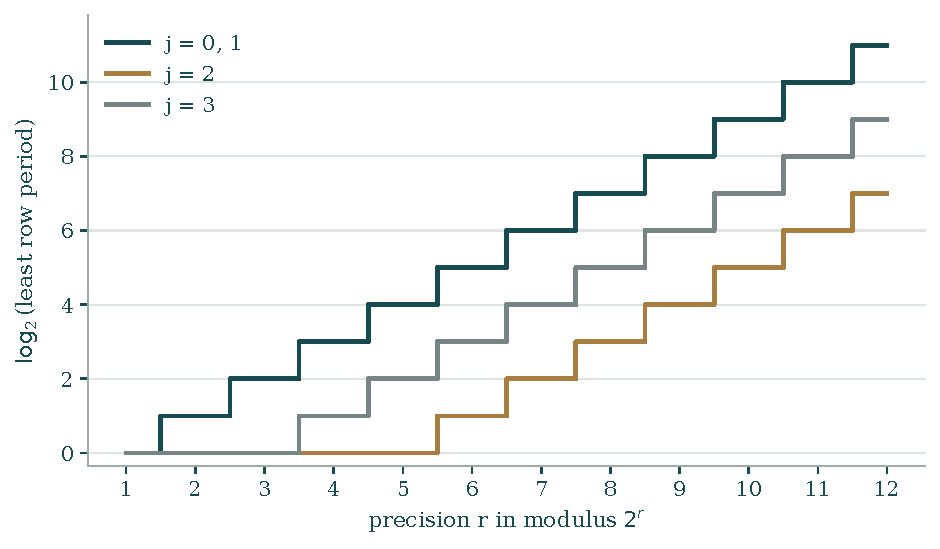
\includegraphics[width=\linewidth]{../figures/periods.pdf}
\caption{Binary logarithms of the least row periods. A height of zero means
period one. These are theorem-derived values, valid at every precision.}
\end{figure}

Modulo $256=2^8$, the least periods are
\[
 (P_0(8),P_1(8),P_2(8),P_3(8))=(128,128,8,32).
\]
In actual Euler degree, multiply by four:
\[
 (512,512,32,128).
\]
For address two, precision at most $2^5$ already has row period one. Its
Euler coefficients all lie in $2+32\mathbb Z_2$. Further precision resolves
additional dyadic digits within that residue class.

The original rank-four conjectural shift has row step $2^{r-1}$. It remains
a valid period for every address, but addresses two and three usually admit
shorter periods. The sharp theorem identifies the shortest one.

\clearpage
\section{A full period visits every allowed residue}

For each address the exact interpolation image is
\[
 E^{(4,j)}(\mathbb Z_2)=j!+2^{B_j}\mathbb Z_2.
\]
When $r>B_j$, a least period lists every residue in this coset modulo $2^r$
exactly once. The following figure checks this assertion by exact arithmetic
at precision $256$.

\begin{figure}[ht]
\centering
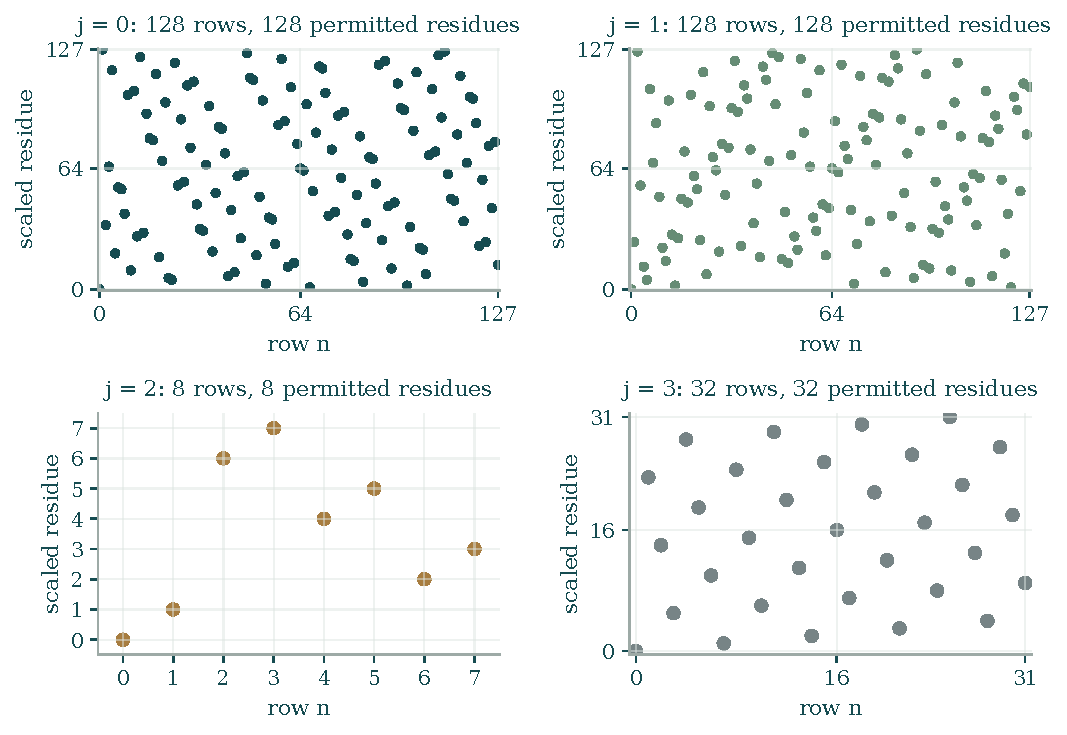
\includegraphics[width=\linewidth]{../figures/residue_permutations.pdf}
\caption{Exact residue permutations modulo $256$. The vertical coordinate is
$y_n=(E_{4n}^{(4,j)}-j!)/2^{B_j}$ modulo $P_j(8)$.
Each panel contains one full least period. Every vertical residue occurs once.}
\end{figure}

No decimal approximation is used to form these residues. The generating
series is inverted modulo $2^{256}$ using odd denominators, then the exact
result is reduced modulo $256$. An independent rational inversion checks the
initial coefficients.

The shapes are permutations, not monotone real functions. Their organizing
property is dyadic distance: agreement in input low bits forces the same
agreement in the scaled output low bits.

\clearpage
\section{Seeing the scaled isometry}

The map
\[
 x\longmapsto \frac{E^{(4,j)}(x)-j!}{2^{B_j}}
\]
is a bijective isometry of $\mathbb Z_2$. Its finite reductions preserve the
number of common low binary digits.

\begin{figure}[ht]
\centering
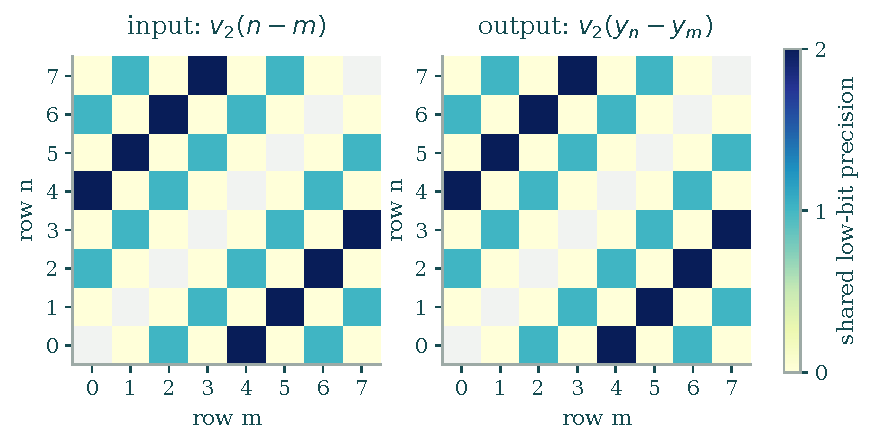
\includegraphics[width=\linewidth]{../figures/isometry_matrices.pdf}
\caption{Address two modulo $256$ gives an eight-element quotient. The
two exact matrices coincide: every pair of distinct rows has the same dyadic
valuation before and after the scale is removed. The diagonal represents
$v_2(0)=+\infty$ and is left blank.}
\end{figure}

If $n-m$ is odd, the rows disagree in their first binary digit and the matrix
entry is zero. If it is divisible by two but not four, they share exactly one
low digit. An entry two means agreement through two low digits.

This structure explains the residue permutation in the preceding section.
At each new precision, every input residue has exactly two lifts. An
isometry distinguishes those lifts at the corresponding output precision.
Starting from the single residue at the scale threshold, induction gives
surjectivity and a unique inverse residue at every finite level.

The finite matrix is an illustration of that proof. Its eight rows alone
would not establish a statement about the whole of $\mathbb Z_2$.

\clearpage
\section{How far the simple metric law extends}

Sharp first-difference laws hold for every address at ranks $2$, $4$, and $8$.
The arrays below give their normalized scales $b_{N,j}$ and original Euler
scales $B_{N,j}=b_{N,j}+v_2(j!)$.

\begin{figure}[ht]
\centering
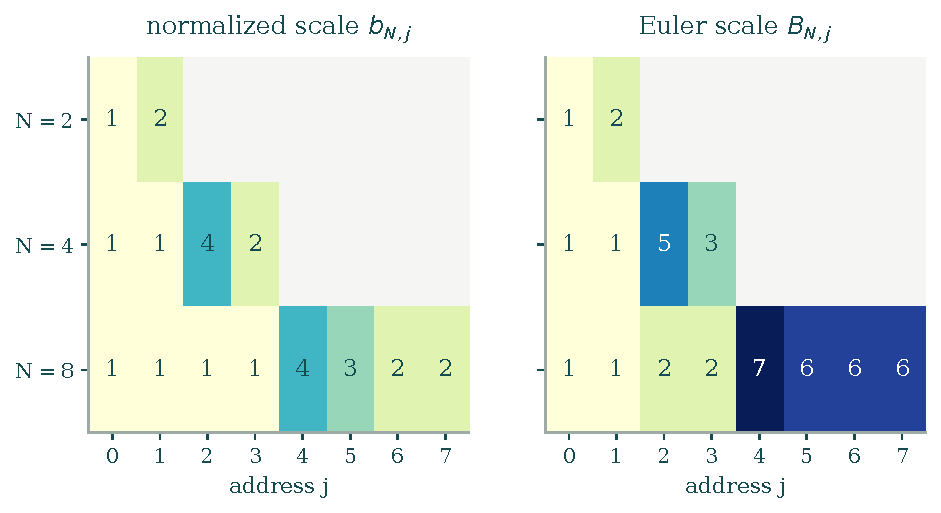
\includegraphics[width=\linewidth]{../figures/rank_scales.pdf}
\caption{Proved scale arrays for the three small ranks. Blank cells are
outside the address range. The Euler normalization contributes the factorial
valuation, which is already substantial at the larger addresses of rank eight.}
\end{figure}

There is also an infinite family: at every $N=2^a\ge4$, all lower-half
addresses $j<N/2$ have normalized scale one. Their Euler scale is
$1+v_2(j!)$.

The same constant-scale proposal fails at some upper-half addresses:
\begin{center}
\begin{tabular}{rrrr}
\toprule
$(N,j)$ & $v_2(C(1)-C(0))$ & Step-two prediction & Actual step-two valuation \\
\midrule
$(16,9)$ & $5$ & $6$ & $7$ \\
$(32,18)$ & $6$ & $7$ & $6$ \\
$(32,19)$ & $5$ & $6$ & $7$ \\
\bottomrule
\end{tabular}
\end{center}

These are exact rational counterexamples to the additional metric proposal.
They do not contradict the universal higher-difference \emph{lower} bound,
which continues to hold at every address of every dyadic rank.

\clearpage
\section{From factorial gain to analytic radius}

At every center $x_0\in\mathbb Z_2$, the interpolations admit ordinary Taylor
series $C_j(x_0+z)=\sum_{d\ge0}a_{j,d}(x_0)z^d$. For positive degrees,
\[
\begin{aligned}
 v_2(a_{j,d}(x_0))&=d &&(j=0,1),\\
 v_2(a_{2,d}(x_0))&\ge\max\{2d+\lfloor d/2\rfloor,\ d+3\},\\
 v_2(a_{3,d}(x_0))&\ge d.
\end{aligned}
\]
At address two equality with $5d/2$ holds along every power-of-two degree
$d\ge4$.

\begin{figure}[ht]
\centering
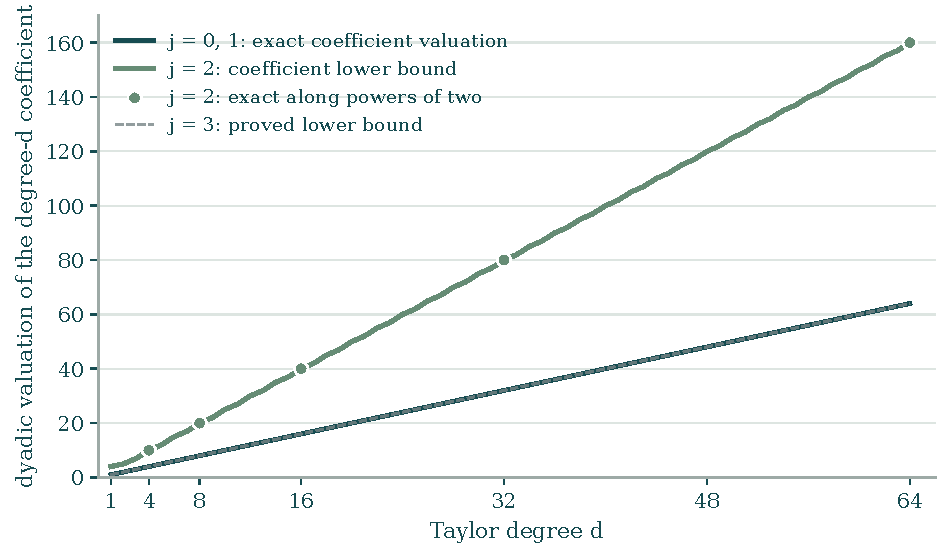
\includegraphics[width=\linewidth]{../figures/analytic_slopes.pdf}
\caption{The Taylor coefficient precision slopes. The degree-zero
coefficient is excluded. Marked address-two degrees belong to an unbounded
proved equality family, rather than a finite observed pattern.}
\end{figure}

The radius is $2^{\liminf_d v_2(a_d)/d}$ in the normalized dyadic absolute
value. Hence
\[
 R_0=R_1=2,\qquad R_2=2^{5/2},\qquad R_3\ge2.
\]
The exact radius of address three is not asserted. For address two, the
lower bound gives convergence inside the claimed radius and the unbounded
equality family prevents a larger one.

The proof converts the factorial Newton estimates into ordinary Taylor
coefficients with the Stirling relations. Generic continuity or first-order
Lipschitz bounds alone do not supply this analytic conclusion.

\clearpage
\section{Which evidence does which job}

The package has three complementary levels of evidence. They answer
different questions, and the final claims retain those distinctions.

\begin{center}
\begin{tabular}{p{.23\linewidth}p{.34\linewidth}p{.34\linewidth}}
\toprule
Evidence & What it establishes & Scope of the final release \\
\midrule
Lean theorem & The precise formal statement follows from its recorded
dependencies and the accepted foundational axioms. & The completed Nishibuchi
conjecture, earlier Chapter IX theory, and the inherited rank-four ordinary-step,
sharp-period, and isometry results. See the Lean guide for build provenance. \\
\addlinespace
Algebraic proof and audit & A universal mathematical result, subject to the
written proof and its stated inputs. & The new general prime-power transfer,
mixed-step and factorial gains, exact higher-order families, broader dyadic
metric laws, and radius results. \\
\addlinespace
Exact computation & The implemented assertion holds in its recorded finite
domain, or an exact counterexample refutes an extension. & Coefficient
regressions, period illustrations, and sharpness or cancellation checks. \\
\bottomrule
\end{tabular}
\end{center}

The generic theorem uses the integral Hurwitz-series product and reciprocal
induction. The factorial theorem uses divided powers and explicit transforms
of the ordinary Euler and Bernoulli series. The ordinary Euler arithmetic
input is the classical Frobenius congruence, with normalization checked against
Gessel's primary exposition. Address two has a self-contained central-factorial
Bernoulli argument. Addresses one and three use the proved tangent and
cotangent transfers.

The broad exact regression through row $512$ contains more than $1.8$ million
bounded difference assertions. Smaller later runs test the strengthened
address-two filtration and the exact mixed parity law. Their manifests pin
precision, coefficient definitions, input versions, and executed ranges.

The figures in this guide have a separate reproducibility record:
\texttt{sources/generate\_figures.py},
\texttt{figures/exact\_figure\_data.json}, and
\texttt{figures/figure\_manifest.json}. Its exact assertions validate the
illustration data. Theorem-derived curves are explicitly recorded as such.

The new general transfer, mixed-step, factorial, and analytic extension has
not been newly formalized in Lean. The rank-four ordinary-step and sharp-period
results have inherited Lean coverage, as mapped in the companion. Mathematical audits
in this package are internal reviews, not claims of external peer review.

\clearpage
\section{Reading the conclusion at the right strength}

The original quantified Nishibuchi conjecture is completed. The stronger
dyadic result applies without a starting-row threshold, and the rank-four
theory now has factorial precision, exact common-step laws for addresses zero
and one, an infinite exact address-two family, optimal periods, and exact
analytic radii for three addresses.

For a common step, the final congruence to use is
\[
 \Delta_H^k E^{(4,j)}(n)
 \equiv0\pmod {2^{v_2(k!)+k v_2(H)+A_j(k)}},
 \quad n\ge0,\ k,H\ge1,
\]
with
\[
 (A_0,A_1,A_2,A_3)
 =\bigl(k,k,\max\{k+4,2k+\lfloor k/2\rfloor+1\},k+2\bigr).
\]
For different steps, replace $k v_2(H)$ by $\sum_i v_2(H_i)$ in the lower
bound. The address-zero/one equality rule then depends on order parity and the
number of even steps.

\begin{center}
\begin{tabular}{p{.55\linewidth}p{.35\linewidth}}
\toprule
Statement & Final status \\
\midrule
Nishibuchi Conjecture 3.9, all allowed branches & completed as the formal capstone \\
All-row dyadic mixed-difference bound & proved and audited \\
Rank-four factorial and paired bounds & proved and audited \\
All common-step exact valuations, $j=0,1$ & proved at all rows and orders \\
Address-two exact valuations at power-of-two orders & proved for all positive step lists \\
Complete exact address-two formula at other orders & open \\
Complete exact higher-order address-three formula & open \\
Exact address-three analytic radius & open \\
Simple constant metric at every upper-half address & false, with exact witnesses retained \\
Separate Euler-tail universal simplicity problem & open as a distinct research program \\
\bottomrule
\end{tabular}
\end{center}

The remaining questions do not weaken the completed conjecture. They specify
the next boundary of the stronger theory. The main text gives the proofs and
precise dependency statements, while the Lean guide supplies the formal
coverage map and a reproducible route to its recorded checks.

\clearpage\def\AtlasFigDir{../figures/worked}% Shared worked examples. Exact data and figure generation: tools/worked_examples.py.
\begingroup
\ifdefined\IXMainAtlas
\section{Worked arithmetic and lifting atlas}\label{app:worked-atlas}
These examples connect the coefficient calculus with the correction machinery. They instantiate the statements in the main text rather than add new universal claims. Each displayed rational value, residue, and finite reconstruction is checked by the accompanying exact script.
\fi
\newcommand{\AtlasHead}[2]{\ifdefined\AtlasStarted\clearpage\fi\ifdefined\IXMainAtlas\subsection{#1}\else\section{#1}\fi\label{#2}\def\AtlasStarted{1}}
\newcommand{\AtlasImage}[1]{\begin{center}\includegraphics[width=.91\linewidth]{\AtlasFigDir/#1.pdf}\end{center}}
\AtlasHead{Compute the reciprocal before estimating it}{atlas:reciprocal}
For width $N$ and address $j$, the normalized source and its reciprocal are
\[
 G_{N,j}(t)=j!\sum_{n\ge0}\frac{t^{Nn}}{(Nn+j)!},\qquad
 G_{N,j}(t)^{-1}=\sum_{n\ge0}C_{N,j}(n)\frac{t^{Nn}}{(Nn)!}.
\]
Multiplying the two series and clearing the factorials gives an exact triangular recurrence:
\[
 C_{N,j}(0)=1,\qquad
 C_{N,j}(n)=-\frac{\displaystyle\sum_{r=0}^{n-1}
 \binom{Nn+j}{Nr}C_{N,j}(r)}{\binom{Nn+j}{Nn}}.
\]
\AtlasImage{reciprocal_rows}
The table is for $N=4$. The first two address-zero rows illustrate the computation without any valuation estimate:
\[
 C_{4,0}(1)=-1,\qquad
 C_{4,0}(2)=-\bigl(1+\binom84(-1)\bigr)=69.
\]
At address one, the same recurrence yields $C_{4,1}(1)=-1/5$ and $C_{4,1}(2)=121/45$. These are exact rational coefficients, not rounded approximations. The second implementation in the supplied script inverts the ordinary power series first, then multiplies by $(Nn)!$. Agreement between the two constructions checks the factorial placement.

\AtlasHead{The normalization loss is a real boundary}{atlas:normalization}
The original Euler coefficient is $E_{Nn}^{(N,j)}=j!C_{N,j}(n)$. Multiplication by $j!$ changes the available $p$-adic precision. That change cannot be discarded outside the unit-factorial window.

Take $p=3$, $N=6$, $j=3$, and compare rows one and two. Exact inversion gives
\[
 C_{6,3}(1)=-\frac1{84},\quad
 C_{6,3}(2)=\frac{703}{5460},\quad
 C_{6,3}(2)-C_{6,3}(1)=\frac{64}{455}.
\]
\AtlasImage{normalization_loss}
Neither $64$ nor $455$ is divisible by three, so the normalized difference has valuation zero. The original coefficient difference is $3!\cdot64/455=384/455$, of valuation one.

This is the counterexample behind the corrected factorial-loss statement. A bound for the original Euler normalization must lose $v_p(j!)$ when translated to $C_{N,j}$. For $0\le j<p$, that loss is zero. The distinction concerns which sequence the theorem measures, not a numerical weakness of the calculation.

\AtlasHead{Odd primes require the sign twist}{atlas:sign}
The prime-power transfer controls a sign-twisted reciprocal sequence at odd primes. It must not be read as an ordinary-difference theorem for the untwisted coefficients.

At $N=p=3$ and $j=0$, put $A(n)=(-1)^nC_{3,0}(n)$. The first three rows are
\AtlasImage{odd_prime_sign}
The ordinary first difference at row zero is $-1-1=-2$. It is a $3$-adic unit, so an asserted lower bound of one for that difference would be false. The twisted first difference is zero, whose mathematical valuation is $+\infty$. At the next row, the twisted difference is $19-1=18$, of valuation two.

Equivalently, the untwisted sequence is acted on by $T_H=S^H-(-1)^H$, where $S$ advances one row. At odd step one this is $S+1$, not $S-1$. The zero in the example is handled by a zero-safe divisibility statement rather than a finite valuation equality. The explicit sign and the zero convention are both part of the theorem's interface.

\AtlasHead{Newton coordinates turn precision into a finite computation}{atlas:newton}
Let $b_k=\Delta_1^kC_{4,0}(0)$. The first coefficients obtained from the difference triangle are
\[
(b_0,b_1,b_2,b_3,b_4)=(1,-2,72,-33872,60511872).
\]

The exact Newton identity recovers each nonnegative integer row:
\[
 C_{4,0}(n)=\sum_{k=0}^{n}b_k\binom nk.
\]
\AtlasImage{newton_cutoff}
For this address the proved law is $v_2(b_k)=2k-s_2(k)$ for $k\ge1$. Every $k\ge5$ therefore has $v_2(b_k)\ge8$. Since $\binom nk$ is integral, those terms vanish modulo $256$. Thus, for every $n\ge0$,
\[
 C_{4,0}(n)\equiv1+254\binom n1+72\binom n2+
 176\binom n3+128\binom n4\pmod{256}.
\]
The uniform truncation follows from the coefficient theorem. The script separately checks the exact Newton reconstruction and this reduction for rows $0$ through $32$. Those finite checks validate the worked arithmetic without replacing the theorem.

\AtlasHead{A compatible root is built one digit at a time}{atlas:smooth}
Take $F(x)=x^2-7$ over the $3$-adic integers and start with $x_1=1$ modulo three. If $F(x_L)=3^Lr_L$, the next representative has the form $x_{L+1}=x_L+3^Lt_L$. Its correcting digit satisfies
\[
 r_L+2x_Lt_L\equiv0\pmod3.
\]
\AtlasImage{smooth_tower}
For example, $F(1)/3=-2$ and $2x_1=2$, so the next digit is one and $x_2=4$. Then $F(4)/9=1$, again giving digit one and $x_3=13$. At the next stage the residual is divisible by three, so digit zero is correct. A zero digit is not a stalled construction.

Every center remains congruent to one modulo three. Hence $2x_L$ stays a unit, and the correction equation has a unique digit at every stage. The representatives are compatible and their increments are divisible by $3^L$. Completeness gives a limit, and continuity of the polynomial gives a root of $F$. The finite table exhibits the construction. The unit derivative is what supports indefinite continuation.

\AtlasHead{A singular residual can stop a lift}{atlas:blocked}
Now take $F(x)=x^2-3$ at the residue $x=0$ modulo three. The residual is $r=F(0)/3=-1$ and the Jacobian is zero modulo three. The next-digit equation would require
\[
 -1+0\cdot t\equiv0\pmod3,
\]
which has no solution.
\AtlasImage{singular_block}
The three representatives of the old root class modulo nine all leave residual six modulo nine. Thus the root class exists at precision three but does not lift to precision nine. This is an exact obstruction, not failure of an iterative search.

A singular Jacobian alone does not imply failure. For $F(x)=x^2$ at the same center, the residual is zero and all three candidate digits lift to roots modulo nine. The obstruction is the residual class in the cokernel of the actual Jacobian. It is this class, rather than the rank by itself, that decides whether a next lift exists.

\AtlasHead{Separate corrections need not be one shared correction}{atlas:shared}
Consider the two-component system $F(x)=(x,x-3)$ at $x=0$, with $q=3$ and $L=1$. Both components vanish modulo three. After writing a candidate as $y=3t$, its residual vector modulo three is
\[
 \overline r+J\overline t=(0,2)+(t,t)=(t,t-1).
\]
\AtlasImage{shared_obstruction}
The first coordinate can be corrected by $t=0$. The second can be corrected by $t=1$. No digit corrects both. The available residuals are $(0,2)$, $(1,0)$, and $(2,1)$, none of which is $(0,0)$.

The combined Jacobian maps $t$ to the diagonal vector $(t,t)$. Its image is smaller than the product of its coordinate images. Checking the two projected obstructions independently therefore loses the compatibility condition. The common-correction theorem retains the full residual vector and the shared digit space, which is exactly the information needed to detect this failure.

\AtlasHead{A derivative weight can cost one digit of root precision}{atlas:weighted}
Compare the linear equations $F(x)=3x=0$ and $G_A(x)=3x+3^A=0$, where $A\ge2$. Their coefficient difference has $3$-adic valuation $A$, but their roots differ by
\[
 x_A-0=-3^{A-1},\qquad v_3(x_A)=A-1.
\]
\AtlasImage{weighted_motion}
The derivative has valuation one. Solving the correction equation divides by three, so one digit of coefficient precision is lost in root displacement. The calculation is exact for every displayed $A$ and also follows immediately from the two linear equations.

This example explains why weighted lifting and deformation estimates track a Jacobian loss rather than silently treating every invertible derivative over $\mathbb Q_p$ as a unit over $\mathbb Z_p$. A valuation-zero derivative would not incur this particular loss. Nonlinear systems additionally require their stated neighborhood, residual, and right-inverse hypotheses.

\medskip\noindent\textbf{Reproducibility.} The eight examples use exact rational and integer arithmetic in \nolinkurl{tools/worked_examples.py}. The release record states the executed finite ranges. This atlas adds no Lean endpoint and changes no formal claim in the companion.
\endgroup

\end{document}
